% Source: http://www.brian-amberg.de/uni/poster/
\documentclass[landscape,paperwidth=96in,paperheight=42in,fontscale=0.2]{baposter}
\usepackage[utf8]{inputenc}
\usepackage{fontspec,amsfonts,microtype}
\usepackage{hyperref,url}   % hyperlinks
\usepackage{booktabs}       % professional-quality tables
\usepackage{}      % microtypography
\usepackage{nicefrac,mathtools,xfrac,bm,amsthm}
\usepackage{graphicx}
\usepackage{pgfplots}
\usetikzlibrary{pgfplots.groupplots}
\pgfplotsset{compat=1.18}
\usepackage{tabularx}
\usepackage{comment}
\usepackage{fnpct}
\usepackage{caption}
\usepackage{comment}
\usepackage[framemethod=tikz]{mdframed}

\DeclareMathOperator*{\minimize}{minimize}
\renewcommand{\familydefault}{\sfdefault}

\usepackage{enumitem}\setlist{nolistsep,leftmargin=*}
\usepackage{graphicx}

\usepackage{tikz}
\usetikzlibrary[topaths]
\newcount\mycount

\setmainfont{Lato}[
  SizeFeatures={Size=18},
]
\newfontfamily\titlefont{Raleway-SemiBold}[
  Path = ./fonts/raleway/,
  SizeFeatures={Size=32},
]
\newfontfamily\headerfont{Raleway-Bold}[
  Path = ./fonts/raleway/,
  SizeFeatures={Size=17},
]

\definecolor{headerColor}{rgb}{0.14, .62, .92}


% Display graphics in pgfplots without deformation: https://tex.stackexchange.com/a/338627
\makeatletter
\newcommand\addplotgraphicsnatural[2][]{%
    \begingroup
    % set options in this local group (will be lost afterwards):
    \pgfqkeys{/pgfplots/plot graphics}{#1}%
    % measure the natural size of the graphics:
    \setbox0=\hbox{\includegraphics{#2}}%
    %
    % compute the required unit vector ratio:
    \pgfmathsetmacro{\xfactor}{\wd0/(\pgfkeysvalueof{/pgfplots/plot graphics/xmax} - \pgfkeysvalueof{/pgfplots/plot graphics/xmin})}%
    \pgfmathsetmacro{\yfactor}{\ht0/(\pgfkeysvalueof{/pgfplots/plot graphics/ymax} - \pgfkeysvalueof{/pgfplots/plot graphics/ymin})}\yfactor%
    % The smaller of the unit vectors should be 1, so the other needs to be scaled appropriately
    \pgfmathsetmacro{\xunit}{\xfactor<\yfactor ? 1 : \xfactor/\yfactor}
    \pgfmathsetmacro{\yunit}{\xfactor<\yfactor ? \yfactor/\xfactor : 1}
    %
    % configure pgfplots to use it.
    % The \xdef expands all macros except those prefixed by '\noexpand'
    % and assigns the result to a global macro named '\marshal'.
    \xdef\marshal{%
        \noexpand\pgfplotsset{unit vector ratio*={\xunit\space \yunit}}%
    }%
    \endgroup
    %
    % use our macro here:
    \marshal
    %
    \addplot graphics[#1] {#2};
}   
\makeatother


\begin{document}

\begin{poster}{
    %grid=true,
    colspacing=.5in,
    headerColorOne=headerColor, borderColor=headerColor,
    headerborder=none, headershape=rectangle,
    headershade=plain, headerFontColor=white, textborder=none,
    background=plain, bgColorOne=white, boxshade=none,
    headerheight=0.15\textheight,
    headerfont=\headerfont,
    columns=3
  }{
    
\includegraphics[height=0.11\textheight]{images/neurips-logo}
  }{
    {{\titlefont The Pitfalls of Regularization in Off-Policy TD Learning }}
  }{\vspace{2mm}\large
    Gaurav Manek, J. Zico Kolter \\
    School of Computer Science, Carnegie Mellon University \\
    \texttt{<gmanek, zkolter>@cs.cmu.edu}
  }{
\includegraphics[height=0.11\textheight]{images/cmu-logo}}

  \headerbox{Off-Policy TD Learning is Unstable}
  {name=intro,column=0,row=0}{% Highlight Box
\definecolor{teal}{rgb}{0.99,0.37,0.53}
\newmdenv[innerlinewidth=0.5pt, roundcorner=4pt,linecolor=teal,backgroundcolor=teal,innerleftmargin=6pt,
    innerrightmargin=6pt,innertopmargin=6pt,innerbottommargin=6pt,leftmargin=-9pt,rightmargin=-9pt]{mybox}

Temporal Difference (TD) learning estimates the value function of a Markov Reward Process (MRP) using samples of successive differences. This is done with the Bellman equation:
\begin{center}
    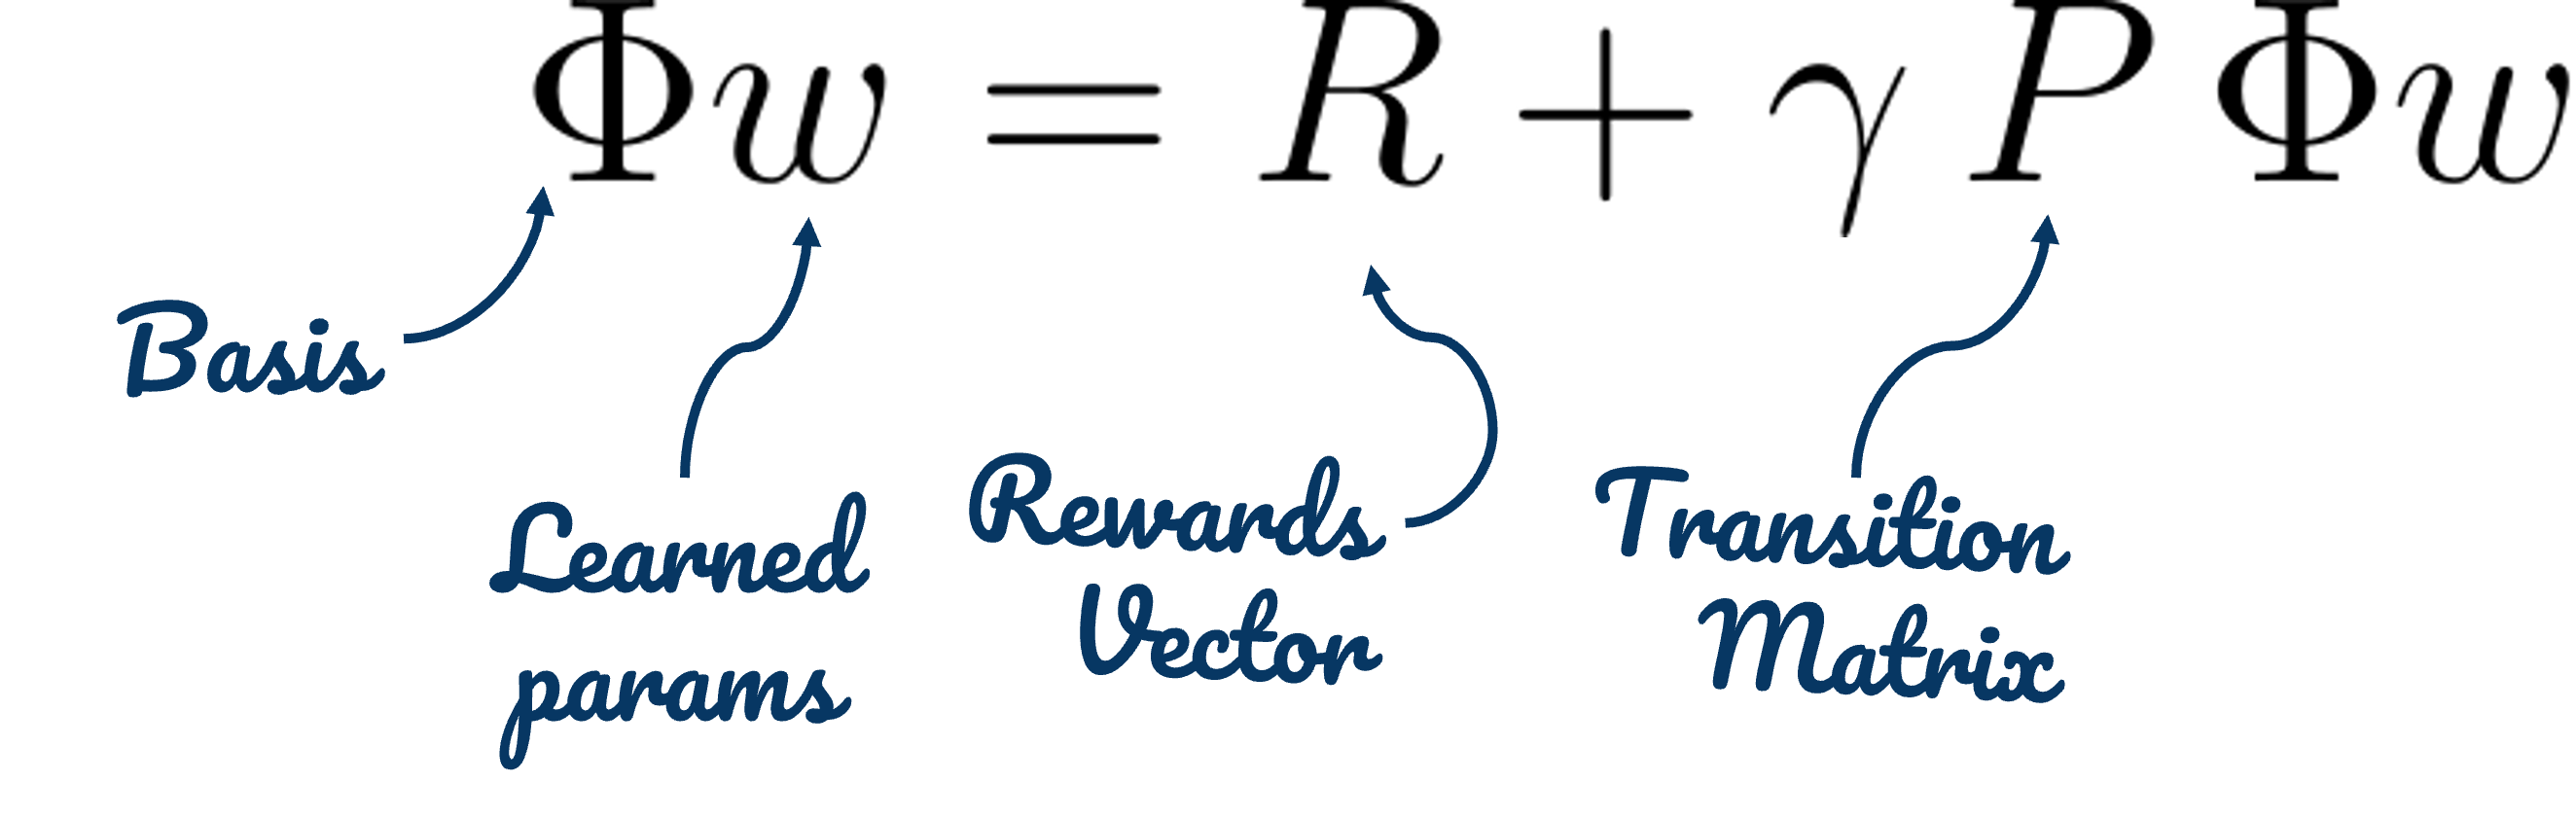
\includegraphics[scale=0.4]{parts/intro/bellman}
\end{center}\vspace{-.1in}
TD may learn arbitrarily bad value functions under \emph{Deadly Triad} conditions:
bootstrapping (learning from your own output),
function approximation, and
off-policy updates.
\vspace{-.11in}
\begin{center}
    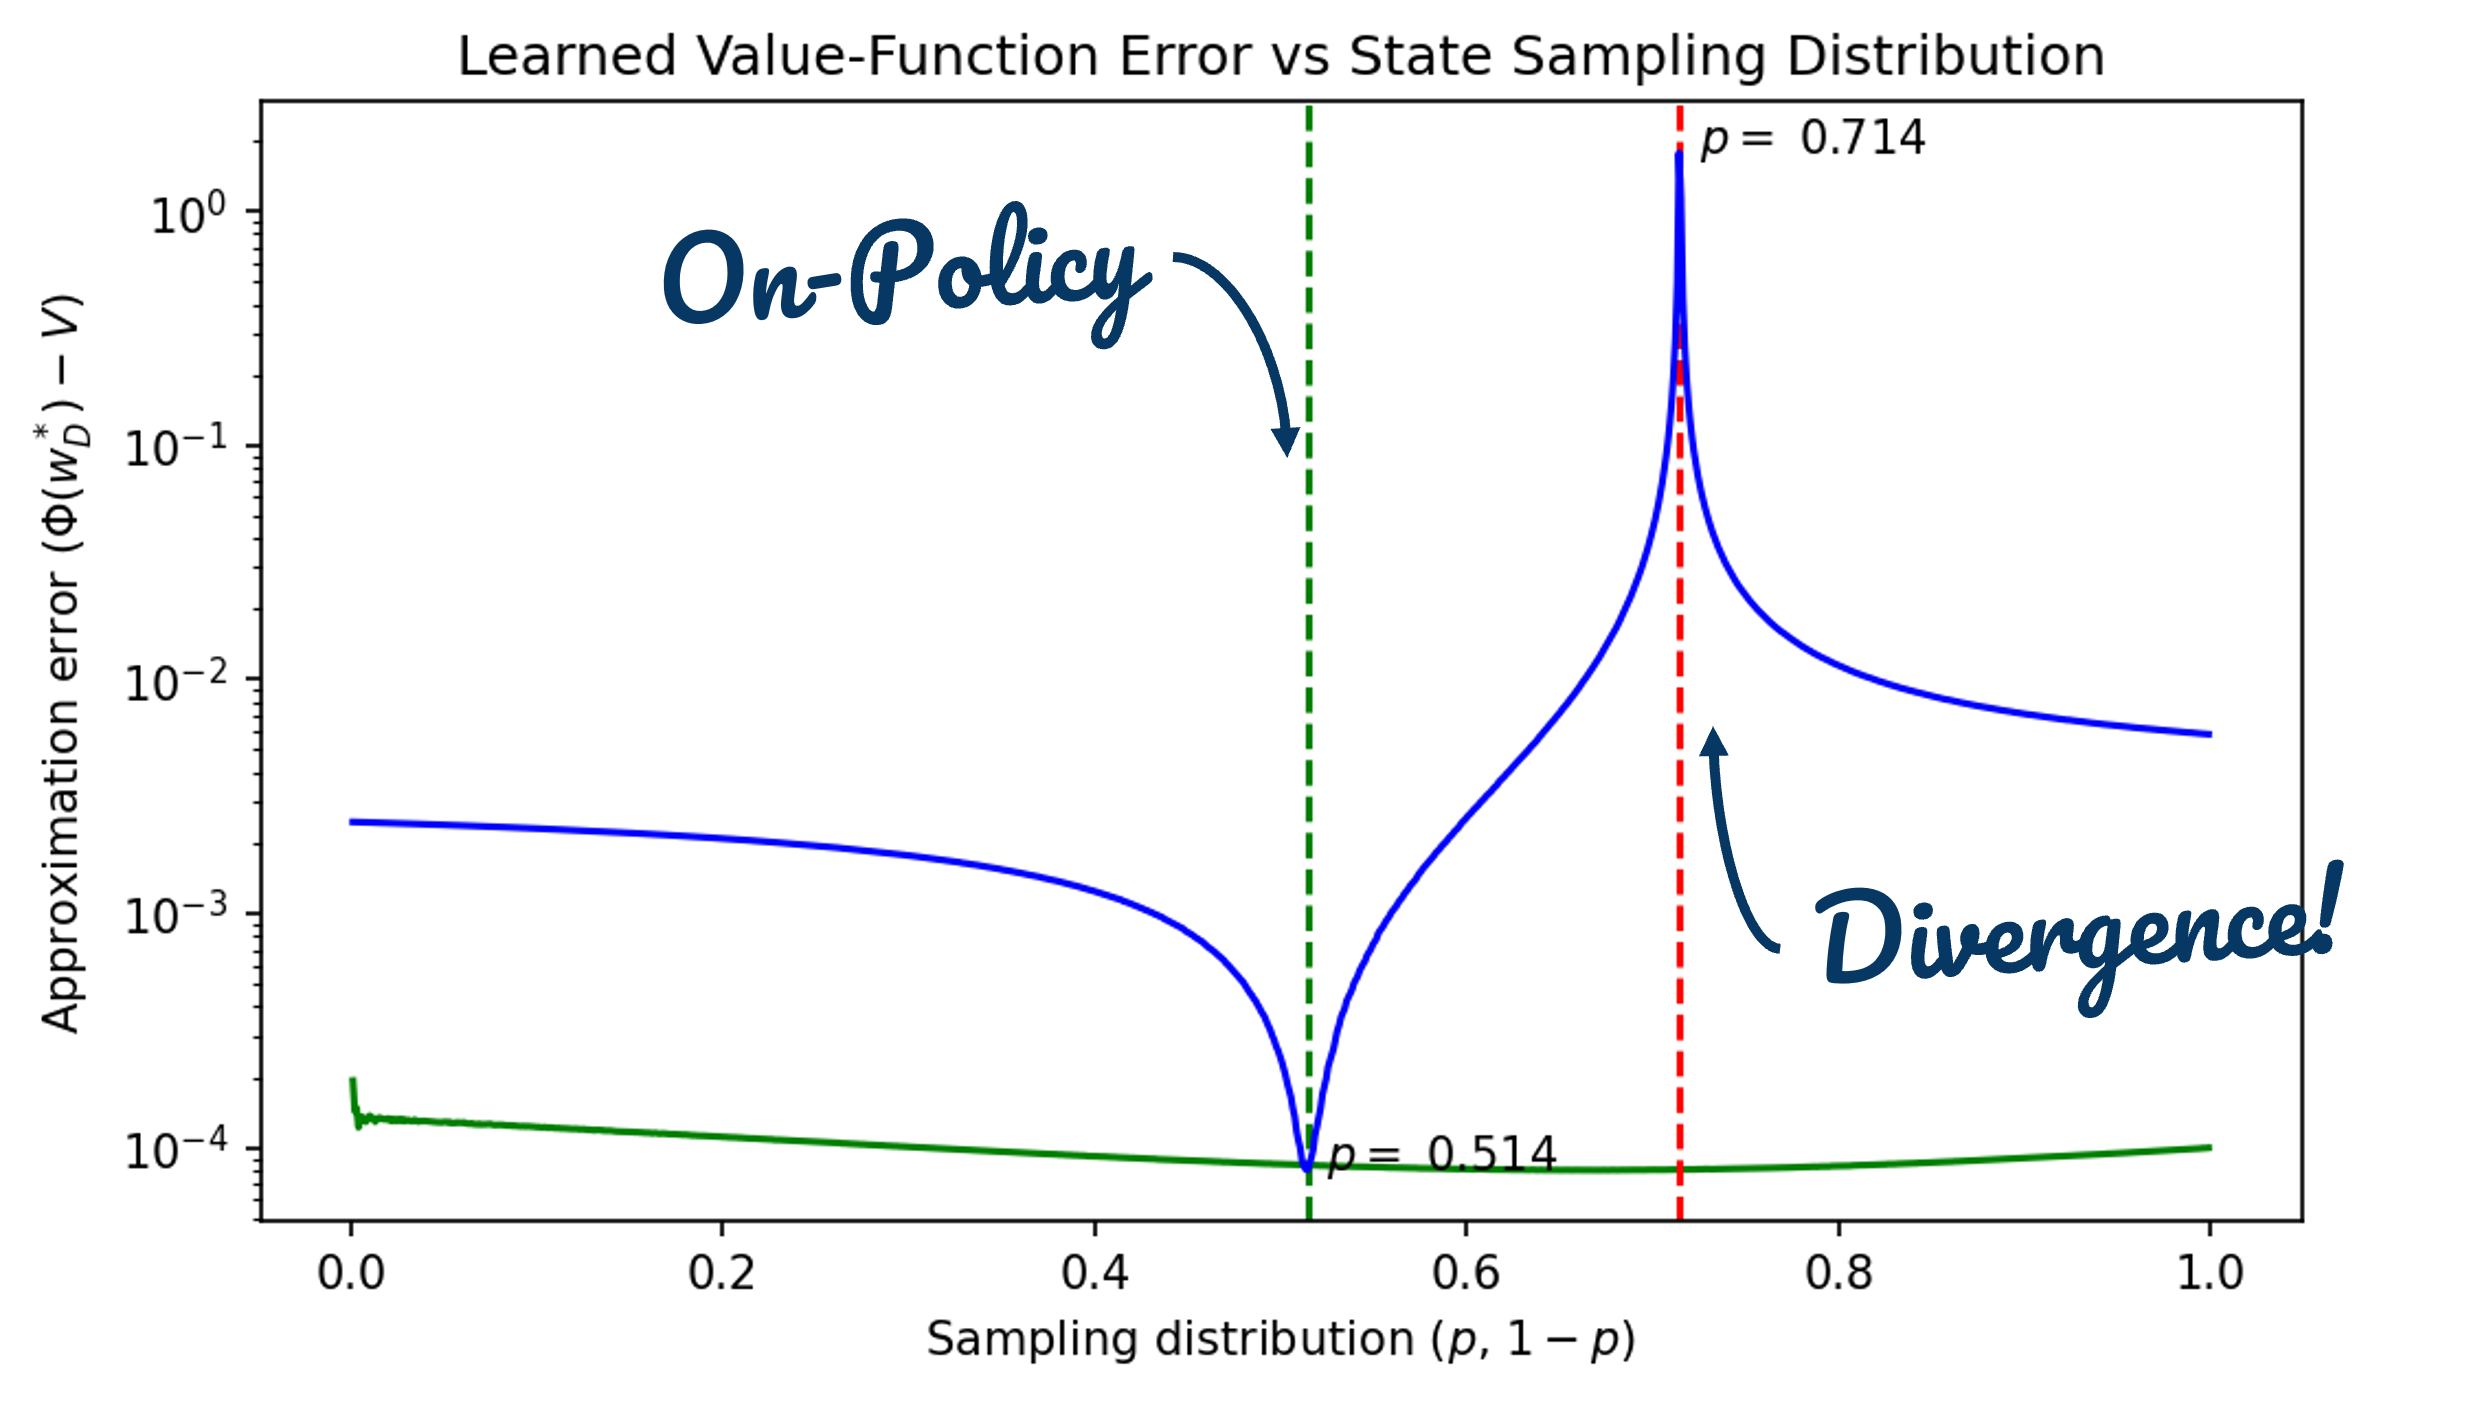
\includegraphics[scale=0.4]{parts/intro/threestatedivergence}
\end{center}\vspace{-.1in}
Regularization is a popular mitigation, and is supposed to work like this:
\begin{center}
    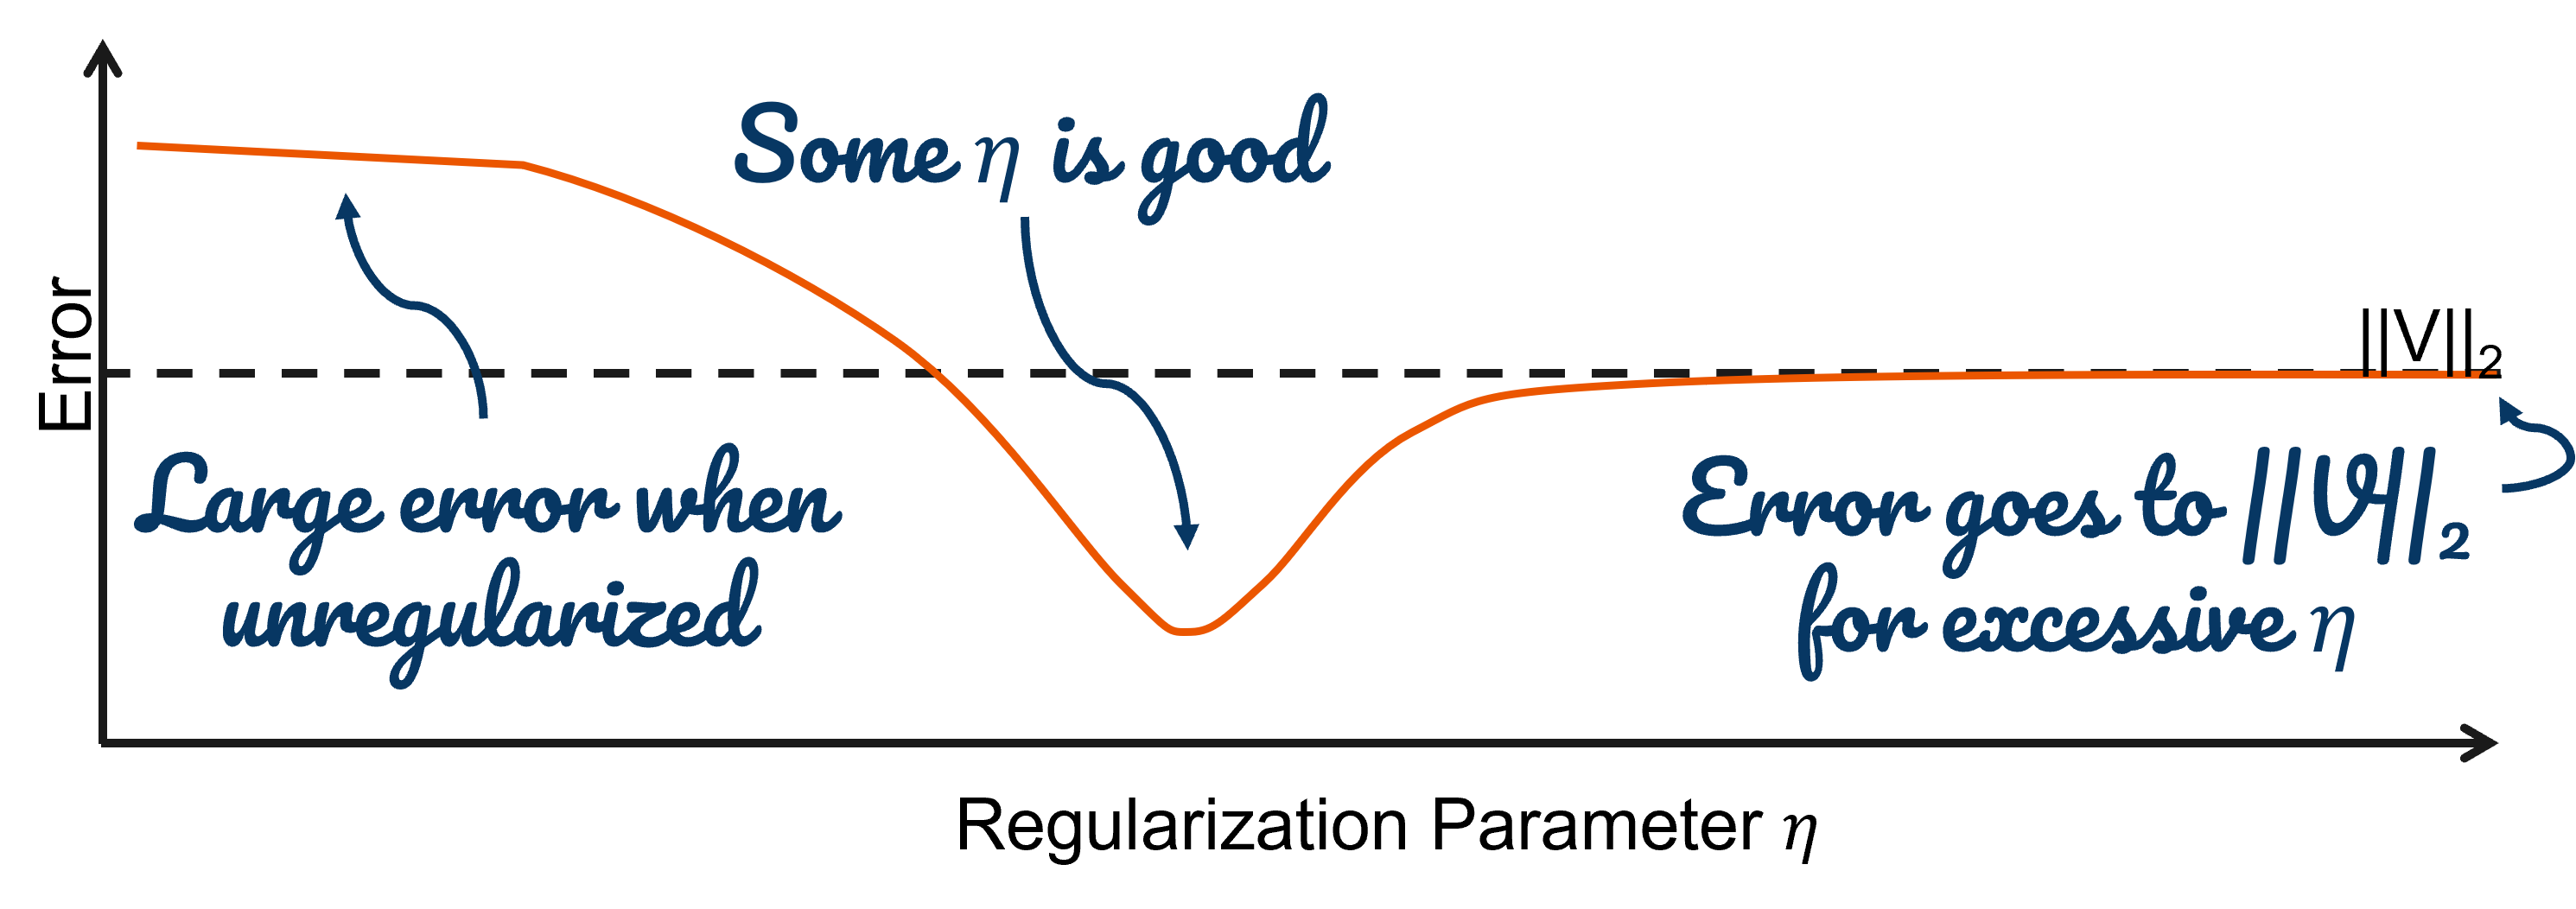
\includegraphics[scale=0.4]{parts/intro/regworks}
\end{center}
\begin{mybox}
    {\headerfont Regularization doesn't always work!}
    \vspace{.5em}
    {\large
        \begin{enumerate}
            \item Models may be \emph{vacuous}.
            \item Regularizing TD is \emph{not monotonic}.
            \item Emphatic models are \emph{not immune}.
        \end{enumerate}
    }
    \vspace{.5em}
\end{mybox}}

  \headerbox{\#1: Models may be \textit{vacuous}}
  {name=vacuous,column=1,row=0}{% Highlight Box
oral Difference (TD) learning is the process of estimating the value of each state using the differences in the value of successive states. This is done with the Bellman equation:
\begin{center}
    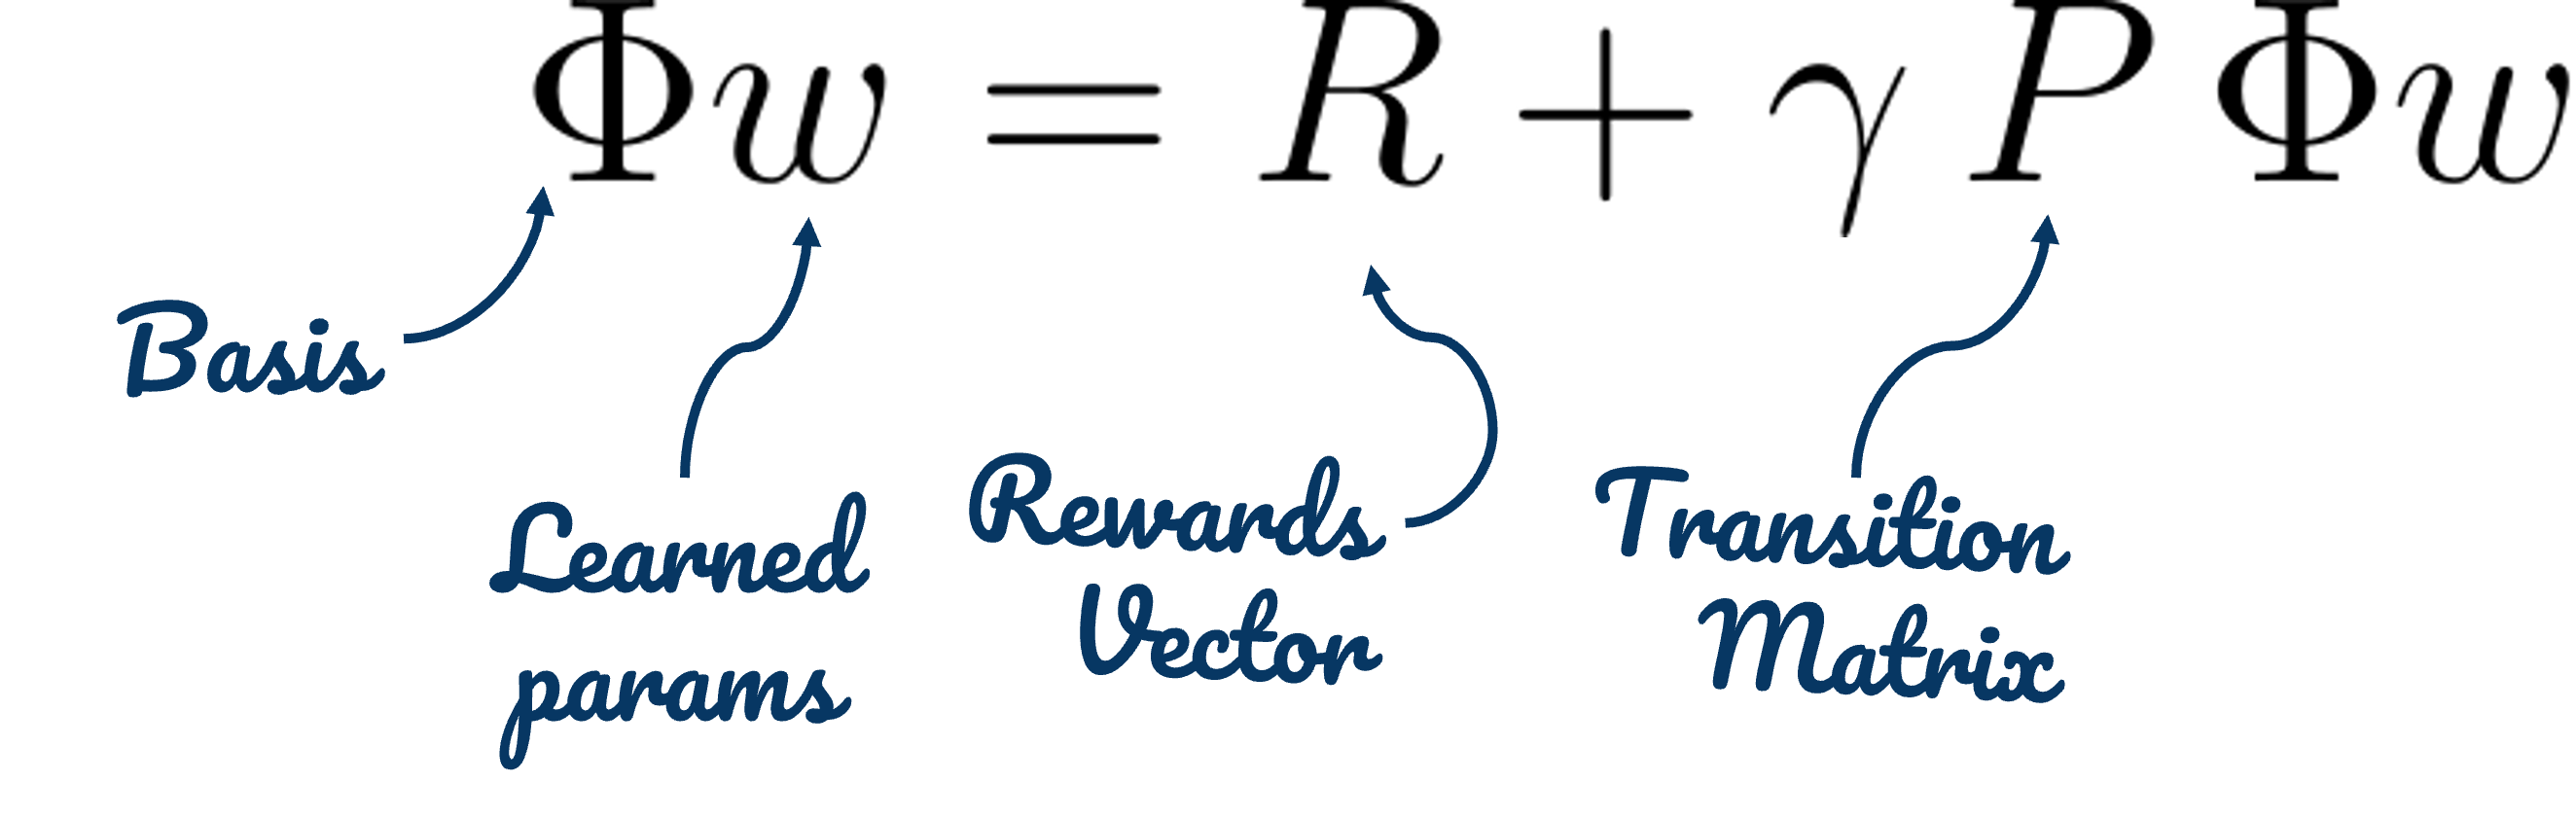
\includegraphics[scale=0.4]{parts/intro/bellman}
\end{center}
TD may learn arbitrarily bad value functions under the \emph{Deadly Triad} conditions:
}

  \headerbox{\#2: Regularization is \textit{not monotonic}}
  {name=nonmonotonic,column=1,below=vacuous}{Fully-supervised regularization monotonically shrinks the learned value function. Bootstrapped regularization is recursively applied, so \textbf{the value function may counterintuitively increase with $\eta$.}
\vspace{-.17in}
\begin{center}
    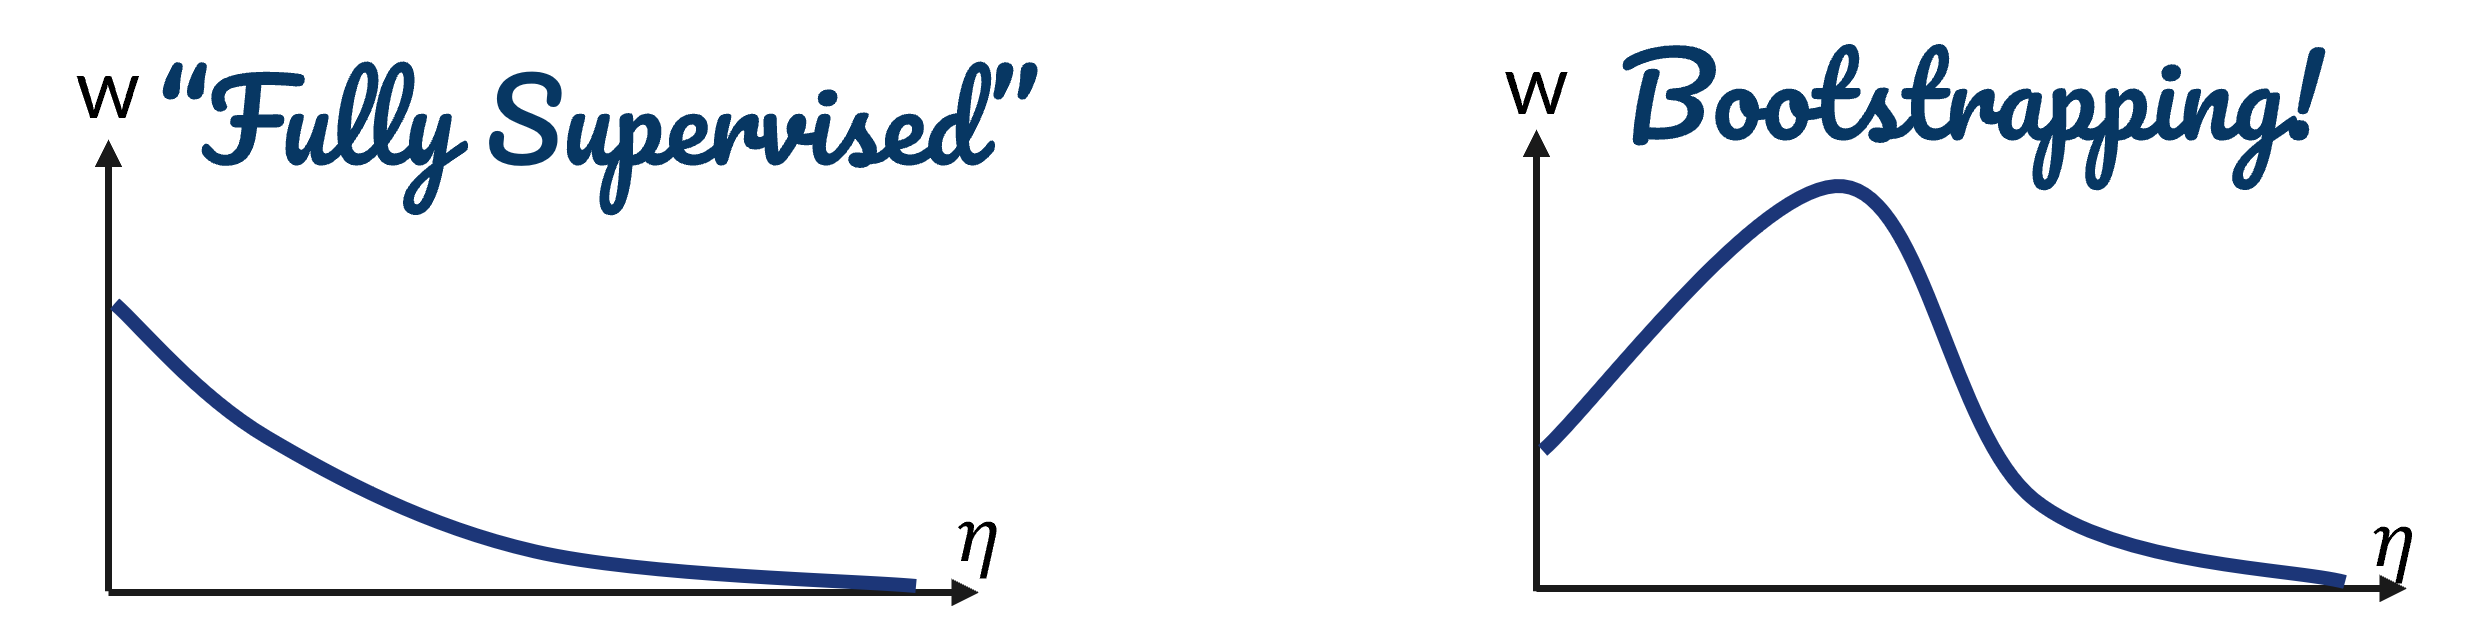
\includegraphics[scale=0.4]{parts/nonmonotonic/illus.png}
\end{center}
\vspace{-.07in}
TD learning may diverge at specific $\eta$, possibly multiple values. For example:
\vspace{-.07in}
\begin{center}
    \hspace*{1in}
    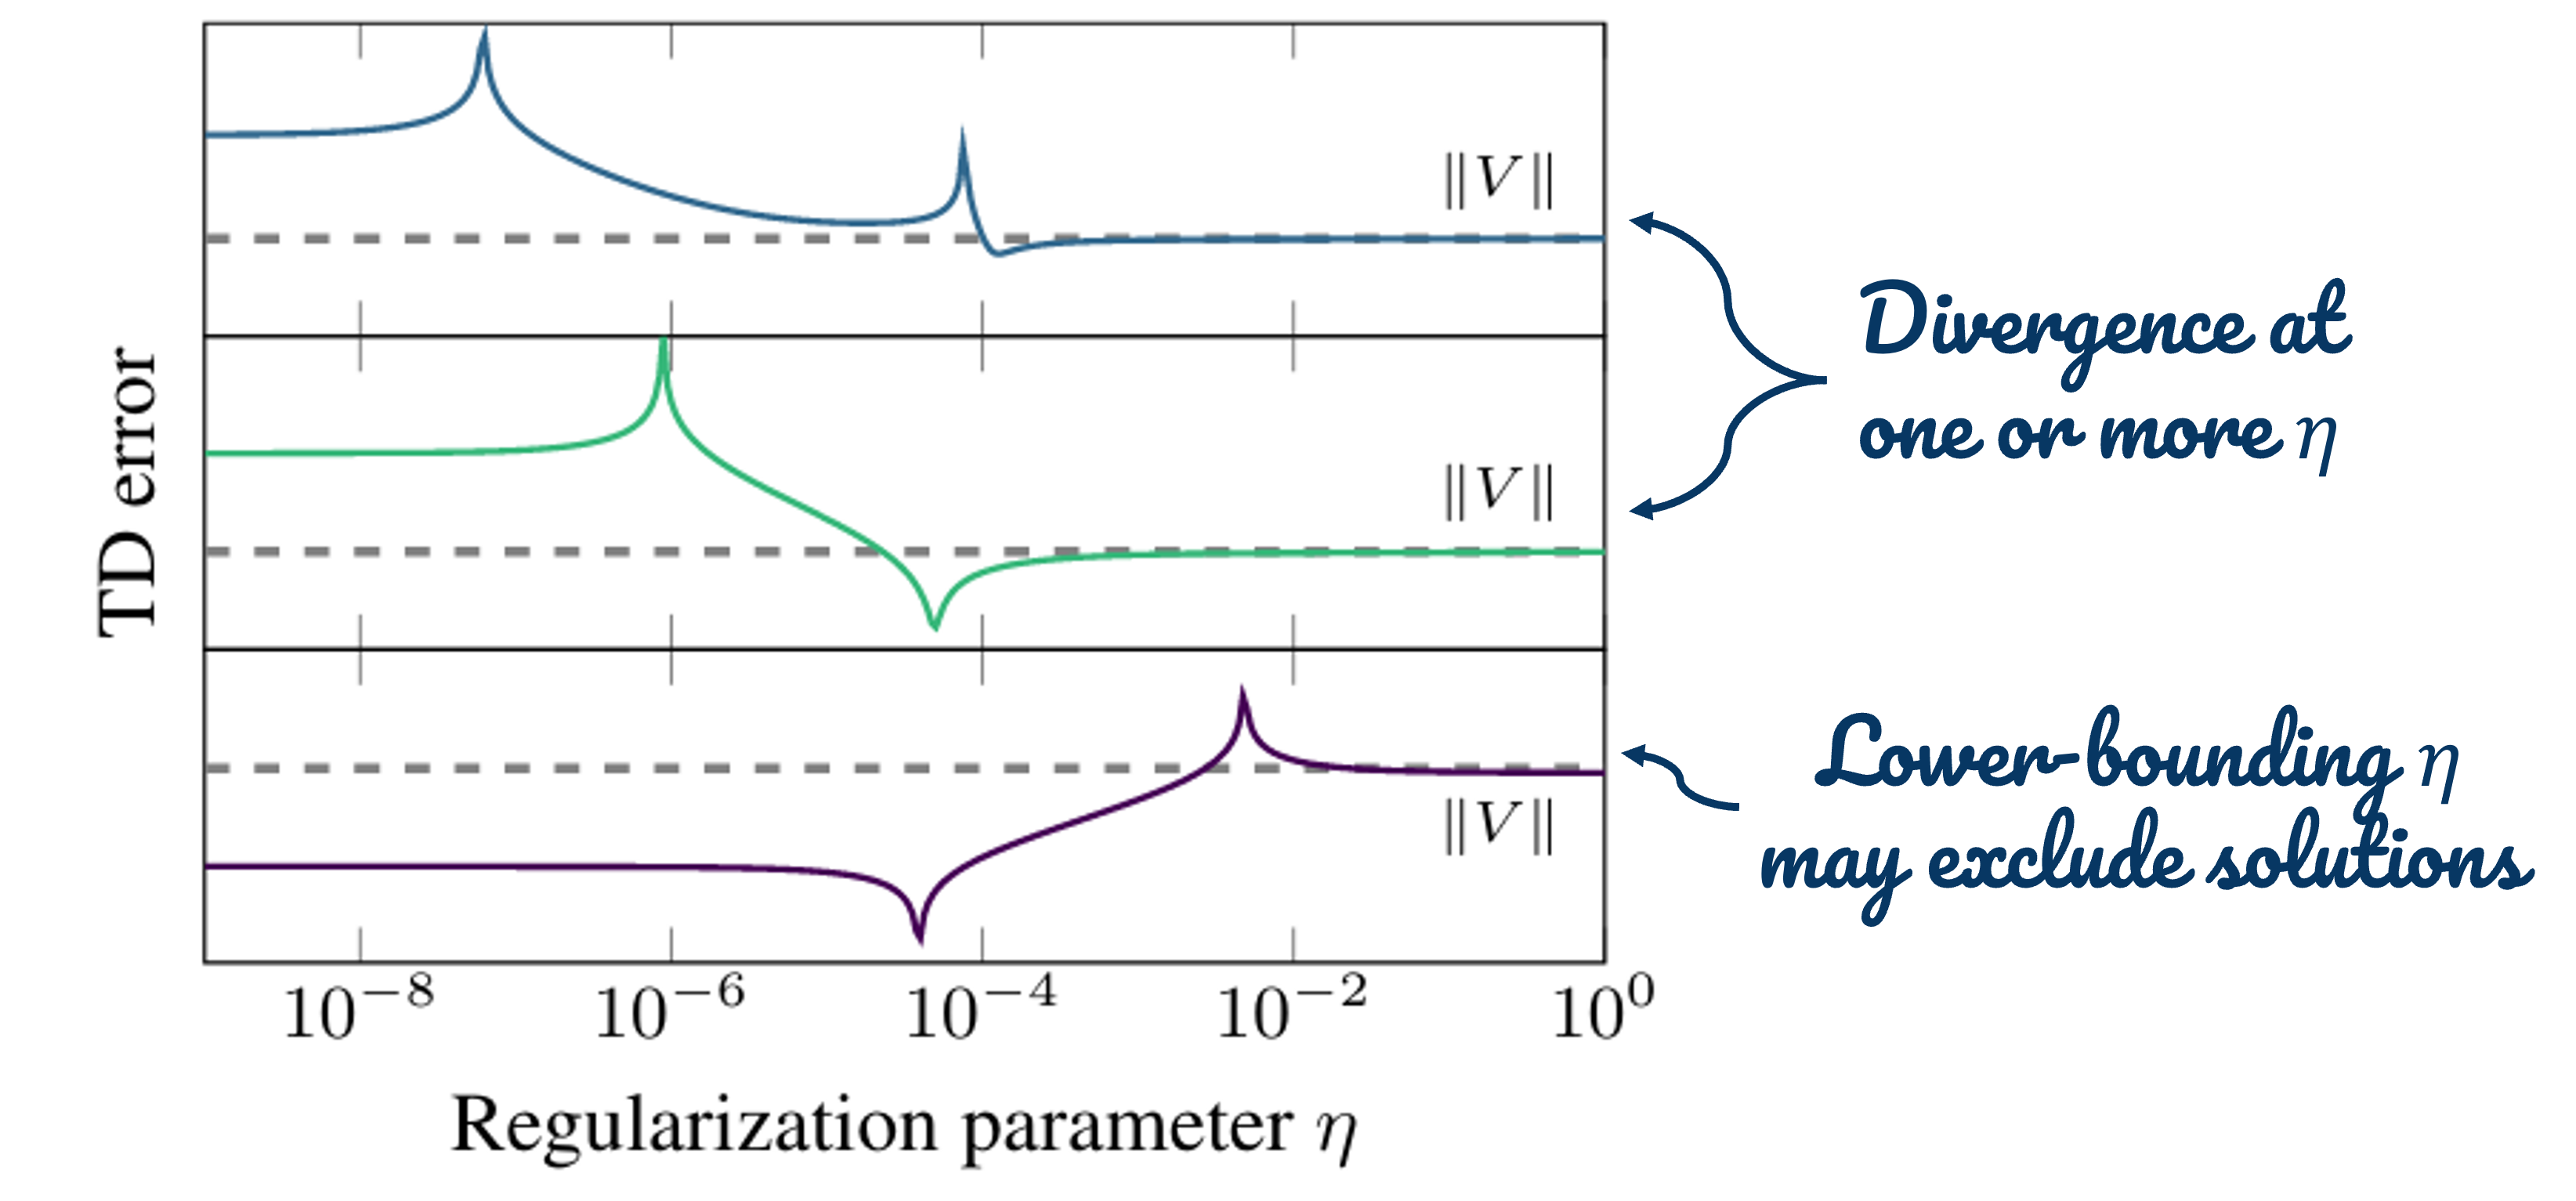
\includegraphics[scale=0.4]{parts/nonmonotonic/threeex.png}
\end{center}
\vspace{-.07in}
A common fix is to assume TD learning behaves ``almost-PSD'' and so lower-bound $\eta$. This assumption is dangerous: it may restrict us to a domain in which TD learning is vacuous.
}

  \headerbox{\#3: Regularization induces divergence in NNs}
  {name=nn,column=2,row=0}{\begin{center}
    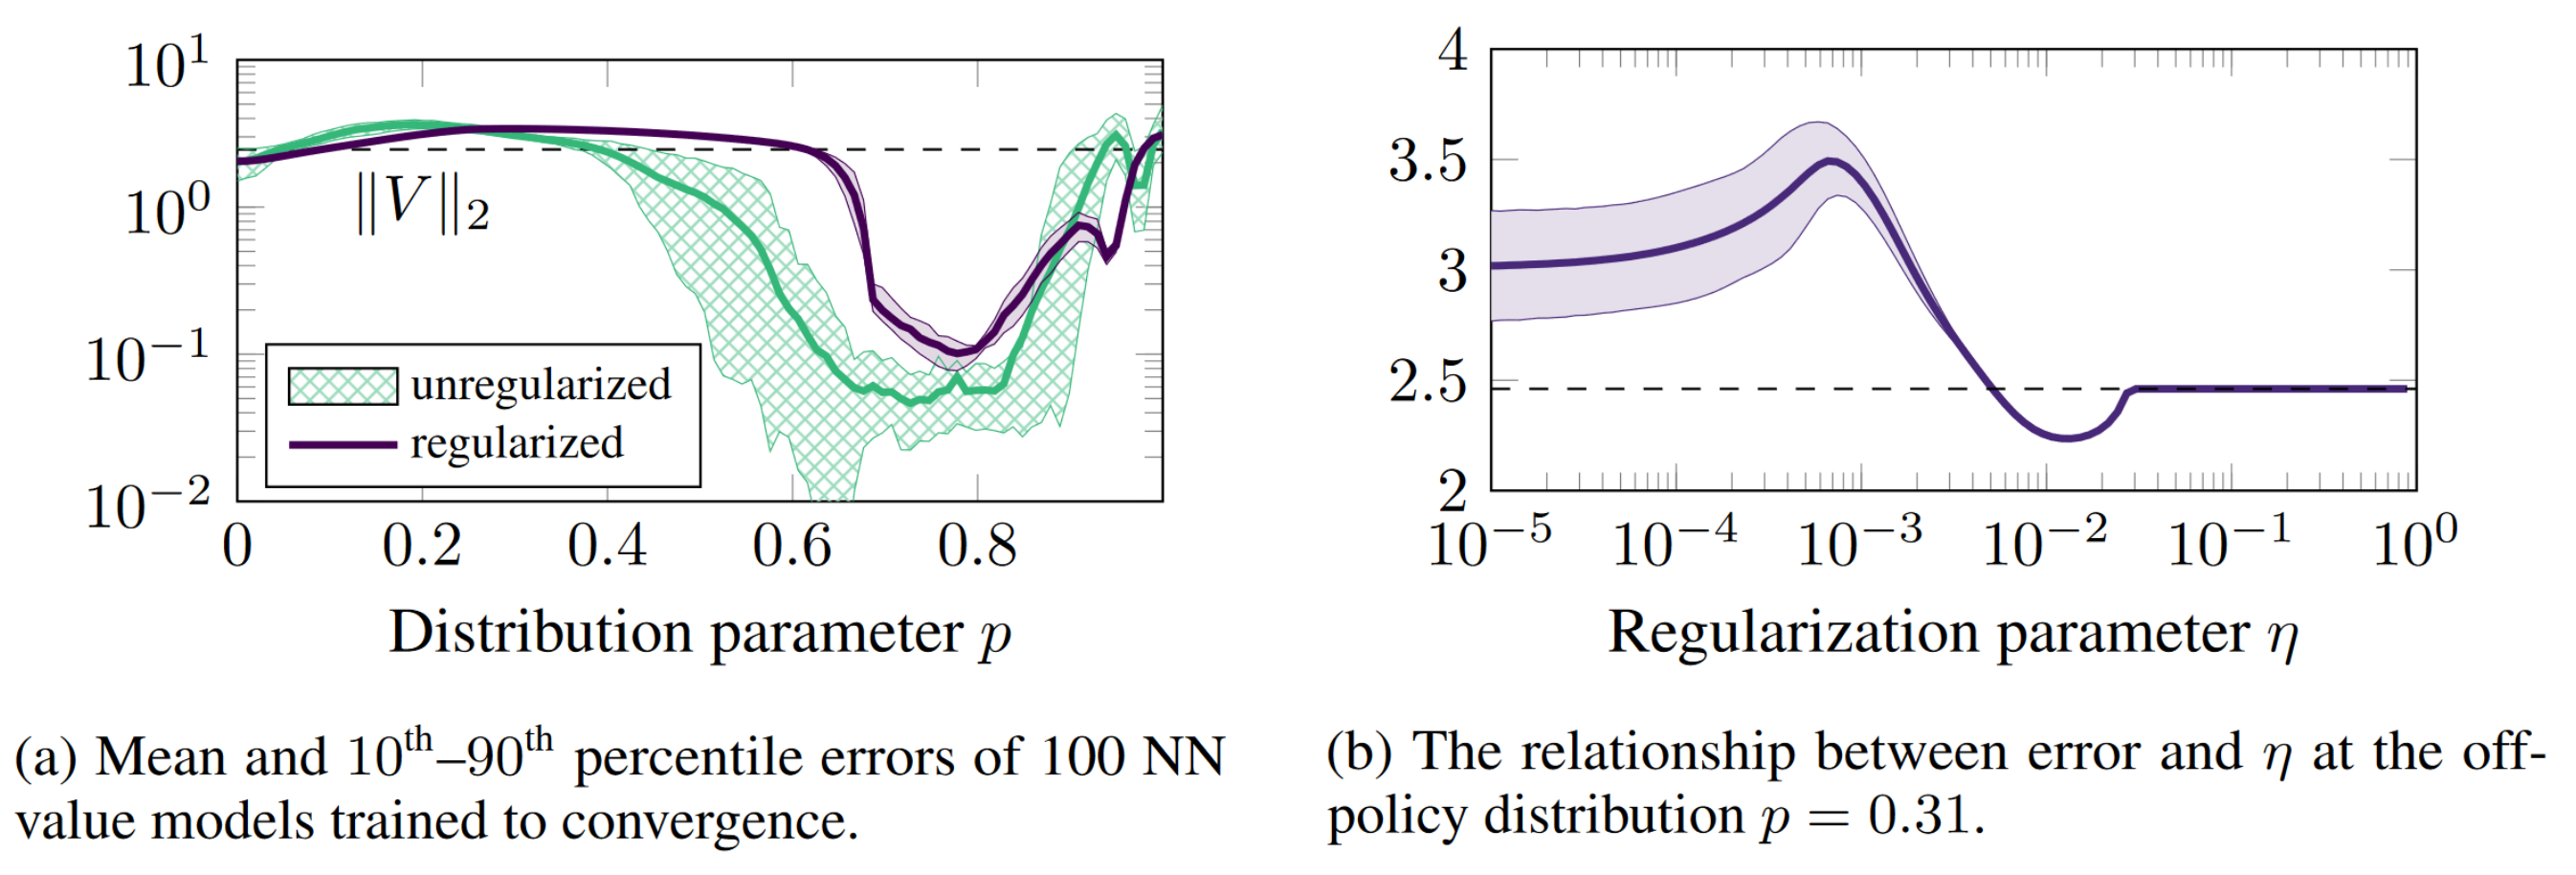
\includegraphics[scale=0.4]{parts/nn/nn2.png}
\end{center}
\vspace{-.11in}
These problems also happen with neural networks.
In (a) we show that NNs may be vacuous for some off-policy distributions. In (b) we show that regularization is non-monotonic.
\vspace{-.7in}
}

  \headerbox{\#4: Emphatic-TD can't fix this.}
  {name=emphatic,column=2,below=nn}{Emphatic-TD (ETD), proposed by Sutton et al. in 2015, is the most promising way to mitigate off-policy training instability. It works by estimating the transitive dependency between states (called the \emph{followon trace}) and uses that to reweight TD updates to appear on-policy.

Estimating the followon trace is very difficult. Modern ETD algorithms do this using a form of reversed TD, which makes it vulnerable to regularization bias.
\begin{center}
    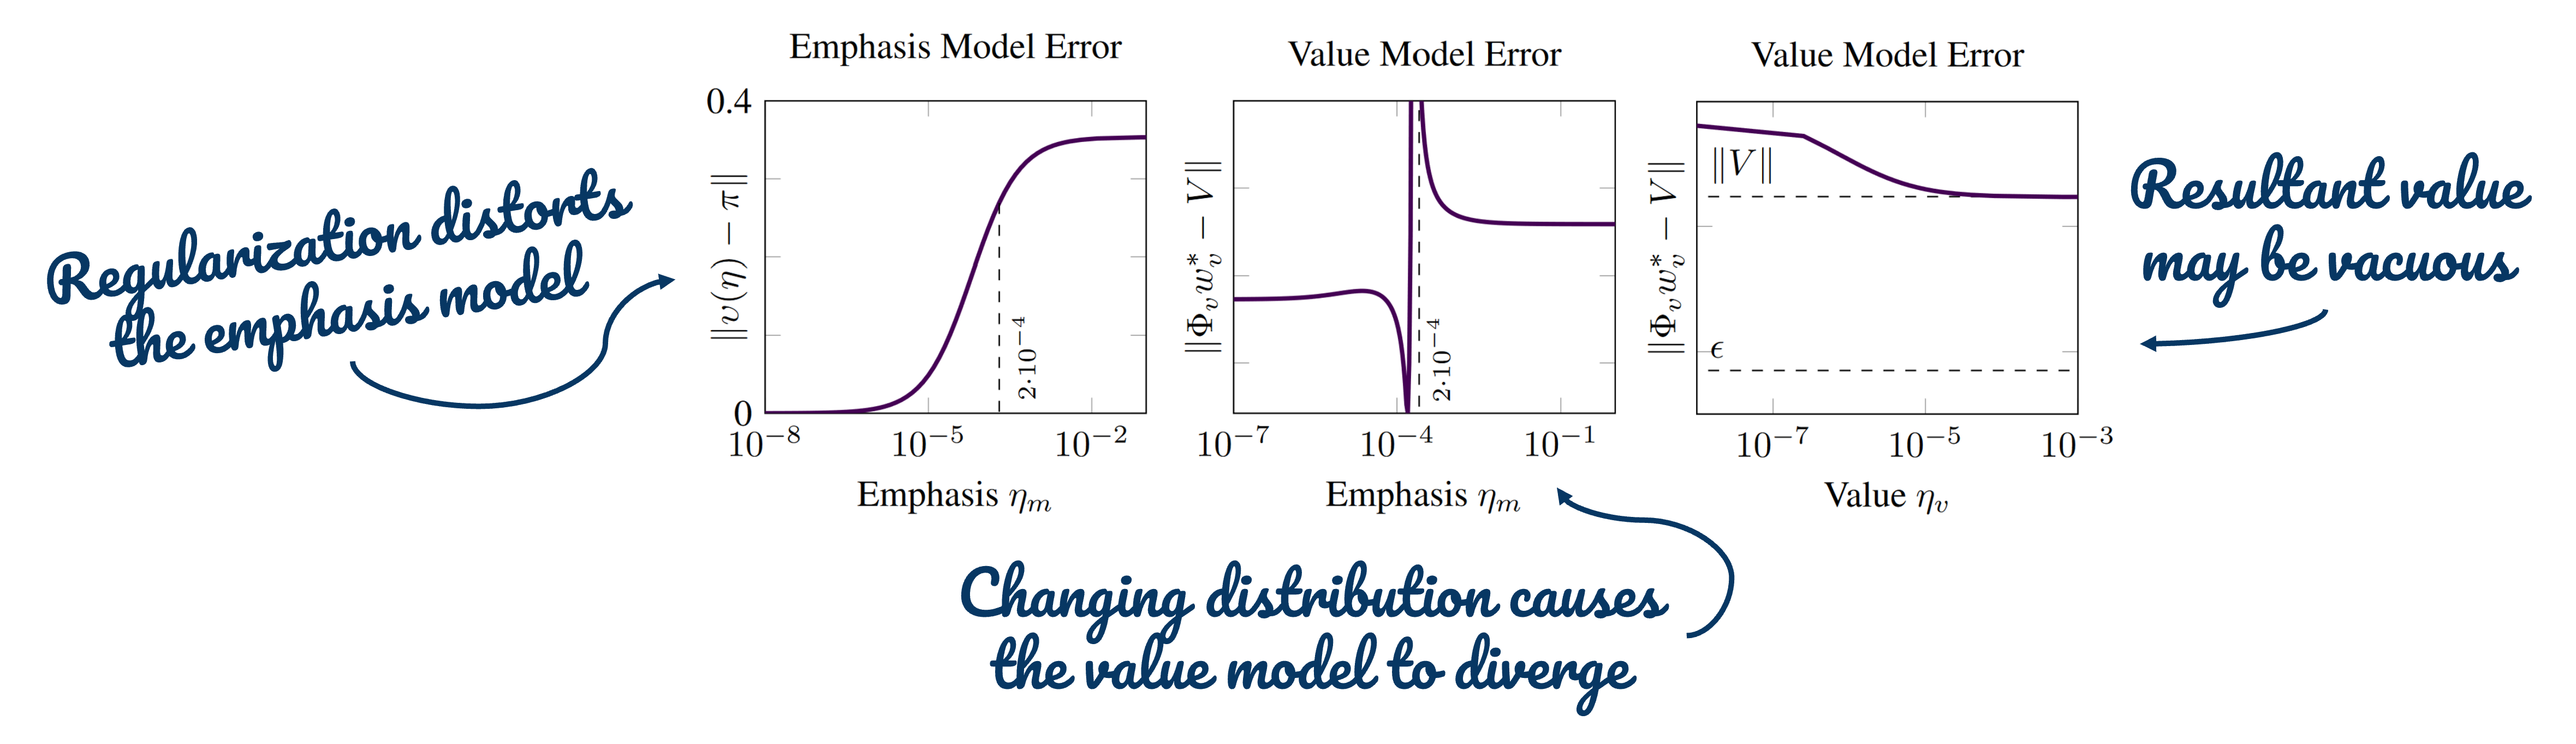
\includegraphics[scale=0.4]{parts/emphatic/emphatic.png}
\end{center}
All trained models exhibit a bump in error at similar levels of regularization, showing that this divergence is not an artifact of poor initialization.
}

  \headerbox{What can we do about this?}
  {name=concl,column=2,below=emphatic}{\begin{enumerate}
    \item Try $\eta$ spanning orders of magnitude, or use a changing schedule.
    \item Try different network architectures and initializations.
    \item Train on-policy (or close to it)
\end{enumerate}
}


\end{poster}
\end{document}
